% ---------------------------------------------------------------------------
% Methods + Results draft -- consolidated from the former "Theoretical
% Expectation" and "Measurement Results" sections.
%
% Written against the checked-in pipeline documented in paper/README.md:
%   lib/geometry.py (two_halo_template, band_profile, kappa_band),
%   lib/jackknife.py, stack_single_jk.py, stack_pairs_jk.py,
%   find_and_stack_pairs.py, combine_jackknife.py,
%   combine_filament_jackknife.py, fit_band_covariance.py,
%   fit_sim_template.py, analysis/sim/*.
%
% Conventions:
%   % CHECK  -- a number recorded in the repo (notes, docstrings, figures)
%               but not reproducible from checked-in result files.
%   % TODO   -- a quantity the pipeline produces but whose value is not in
%               the repo at all; fill from the run outputs / Google Doc.
%   % UNVERIFIED -- describes code or results that are not yet supported by
%               checked-in outputs.
%
% Structure: \section{Methods}, \section{Expected signal from the simulation},
% \section{Results}.
%
% ---------------------------------------------------------------------------

\section{Methods}
\label{sec:method}

The data and mock use the same pair selection, pair-frame stacking, halo
control, and band statistic. The observed stacks also include survey weights,
the Planck mask, and random-catalog subtraction. The mock map is periodic and
has zero mean, so the mock stacks are unweighted and require no random-catalog
subtraction. Observed errors use a spatial jackknife over the footprint; mock
errors use blocks of the simulation box.

\subsection{Pair selection}
\label{sec:pairs}

For every galaxy we compute the comoving distance $D_{\rm c}=\chi(z)\,h$ from
its spectroscopic redshift. Two galaxies form a pair if their line-of-sight
and transverse separations,
\begin{equation}
  r_{\parallel} = |D_{{\rm c},1}-D_{{\rm c},2}|, \qquad
  r_{\perp} = \theta_{12}\,\frac{D_{{\rm c},1}+D_{{\rm c},2}}{2},
  \label{eq:separations}
\end{equation}
with $\theta_{12}$ the great-circle angle between them, satisfy
$r_{\parallel}\leq r_{\parallel,{\rm max}}$ and
$r_{\perp,{\rm min}}\leq r_{\perp}\leq r_{\perp,{\rm max}}$. Because
$r_{\parallel}$ is computed from redshifts it is a redshift-space quantity
and includes the pairwise peculiar velocity (Section~\ref{sec:intro}). We
use three transverse bins, $4$--$6$, $9$--$11$, and $18$--$22\,\hinvMpc$,
referred to below as the $5$, $10$, and $20\,\hinvMpc$ samples, with
line-of-sight cuts of $r_{\parallel,{\rm max}}=5\,\hinvMpc$ for the
$5\,\hinvMpc$ sample and $10\,\hinvMpc$ for the other two. The cuts were
fixed on the mock before the observed stacks were examined
(Section~\ref{sec:sim_expect}). Each unordered pair is counted once. A
galaxy may belong to several pairs and we apply no isolation criterion; the
resulting correlation between pairs is handled by the spatial jackknife
rather than by down-weighting. The pair is assigned the comoving distance
$D_{\rm mid}=\chi(\bar z)\,h$ at the mean redshift of its members. Random
pairs are selected from the full random catalogs with the same criteria.

\subsection{Stacking in the pair frame}
\label{sec:stacking}

Each pair defines a local Cartesian frame on the sky: the $X$ axis runs
from galaxy 1 to galaxy 2, with the pair ordered so that $X$ increases with
Galactic longitude, and the $Y$ axis is perpendicular to it. Galaxy 1 and
galaxy 2 sit at $X=\mp r_{\perp}/2$, $Y=0$, at their own separation, so
within a bin the halo positions spread over the bin width. We lay down a
$101\times101$ grid of points spanning $\pm50\,\hinvMpc$ in both
directions, a spacing of exactly $1\,\hinvMpc$ with a grid point at the
midpoint. A grid point $(X,Y)$ is mapped to Galactic coordinates in the
small-angle approximation,
\begin{equation}
  \Delta l\cos b_{\rm c} = \frac{X\cos\phi - Y\sin\phi}{D_{\rm mid}}, \qquad
  \Delta b = \frac{X\sin\phi + Y\cos\phi}{D_{\rm mid}},
  \label{eq:grid_to_sky}
\end{equation}
where $(l_{\rm c},b_{\rm c})$ is the pair midpoint and $\phi$ is the
position angle of the pair axis, defined by
$(\cos\phi,\sin\phi)\propto(\Delta l\cos b_{\rm c},\Delta b)$.
Each sky position is assigned the value of the HEALPix pixel that contains
it. At $N_{\rm side}=2048$ the pixel scale of $1.7\,\mathrm{arcmin}$ is
finer than the grid spacing, which is $2.4\,\mathrm{arcmin}$ at $z=0.55$,
so no interpolation is applied. Masked pixels receive zero weight. The rare
pairs whose grid extends past a Galactic pole are dropped.

The stacked map is the weighted mean at each grid point,
\begin{equation}
  \hat\kappa(X,Y) = \frac{\sum_{i} w_{i}\,m_{i}(X,Y)\,\kappa_{i}(X,Y)}
                         {\sum_{i} w_{i}\,m_{i}(X,Y)},
  \label{eq:stack}
\end{equation}
where $i$ runs over pairs, $w_{i}=w_{1}w_{2}$ is the pair weight
(Section~\ref{sec:data_cmass}), and $m_{i}\in\{0,1\}$ is the mask value at
the sampled pixel. The pair frame has a four-fold symmetry: the two
galaxies are statistically interchangeable, and the sky above and below the
axis is equivalent. We therefore replace the value at $(X,Y)$ by the mean of
the four symmetry-related pixels $(\pm X,\pm Y)$, removing residual
asymmetries between the two members and across the pair axis.

Single galaxies and single random points are stacked in the same way on a
$100\times100$ grid of $1\,\hinvMpc$ cells centered on the object, with the
axes aligned with Galactic longitude and latitude and the weight $w$ of
Equation~(\ref{eq:weights}) multiplied by the lensing-efficiency factor
(Section~\ref{sec:data_cmass}). Because a single stack has no preferred
direction it is symmetrized radially: pixels are averaged in annuli about
the physical center of the grid, which for an even grid lies between the
four central pixels.

\subsection{Joint footprint and random subtraction}
\label{sec:joint}

The North and South caps form a single weighted sample in
Equation~(\ref{eq:stack}). This differs from averaging two per-cap maps:
with $73$ percent of the galaxies in the North, an equal-weight average
would give each Southern galaxy $2.7$ times the influence of a Northern one
and would carry the noisier Southern map into the combined profile at half
weight.
Single galaxies and single randoms are stacked by the same code with the
same weights, and the corrected single map is their difference,
$\hat\kappa_{\rm g}-\hat\kappa_{\rm r}$. The random-point map absorbs the
mean convergence of the footprint and any offset associated with the mask
or the mean field of the reconstruction.

Random pairs are stacked separately for each cap and combined with weights
proportional to the number of pairs in each. The random-pair map is
subtracted from the galaxy-pair map and held fixed in the error analysis.
Its bridge statistic has magnitude at most $4.1\times10^{-5}$ across the
three samples, compared with observed jackknife errors of at least
$2.2\times10^{-4}$.

\subsection{Control for the halo contributions}
\label{sec:control}

The pair stack contains the one-halo and isotropic two-halo contributions of
both members in addition to any anisotropic excess (Section~\ref{sec:intro}).
We model the isotropic part with a control built from the corrected single
stack. Let $P(r)$ be the radial profile of the radially symmetrized
corrected single map, interpolated linearly in radius. The control for a
pair of separation $d$ is the superposition
\begin{equation}
  T(X,Y) = P\!\left(\sqrt{(X-d/2)^{2}+Y^{2}}\right)
         + P\!\left(\sqrt{(X+d/2)^{2}+Y^{2}}\right),
  \label{eq:control}
\end{equation}
evaluated at the bin-center separation on the $101\times101$ pair grid. It
has unit amplitude and no free parameters. We define the residual map as
\begin{equation}
  F(X,Y) = \left[\hat\kappa_{\rm gp}(X,Y)-\hat\kappa_{\rm rp}(X,Y)\right]
           - T(X,Y),
  \label{eq:filament}
\end{equation}
where gp and rp denote the galaxy-pair and random-pair stacks.

The control represents two average CMASS galaxies placed at the pair
positions and subtracts their measured mean isotropic signal. It does not
remove differences between the environments of paired and average galaxies.
Such differences remain in $F$ as residual convergence around the galaxies
and as structure aligned with the pair axis. The single stack includes the
lensing-efficiency weight, whereas the pair stack does not; the control and
pair map therefore have different redshift weights, and the analysis does
not correct this mismatch. The mock is processed with the same control and
band statistic (Section~\ref{sec:sim_expect}). We do not fit the amplitude of
$T$ to the pair stack because fitting axis-aligned structure would allow the
control to absorb the bridge signal. Section~\ref{sec:robust} tests this
effect on the mock.

\subsection{Band statistic}
\label{sec:bands}

Rather than interpret the two-dimensional map pixel by pixel, we compress
$F$ into a profile along the pair axis. For each column $X$ we take the
mean of $F$ in a central band $|Y|\leq1.5\,\hinvMpc$, where a filament
would lie, and in an off-center band $1.5\leq|Y|\leq10.5\,\hinvMpc$ that
brackets it, and form their difference,
\begin{equation}
  B(X) = \langle F(X,Y)\rangle_{|Y|\leq1.5}
       - \langle F(X,Y)\rangle_{1.5\leq|Y|\leq10.5}.
  \label{eq:band}
\end{equation}
The band widths are fixed in comoving units at every separation, so all
three samples use the same physical bands. Rows straddling a band
boundary are given fractional weights equal to the fraction of the row that
lies inside the band, so the statistic does not depend on where pixel edges
fall; on the $101$ grid the bands are three and eighteen whole rows. The
difference suppresses components that vary slowly with $Y$ and removes an
offset shared by both bands. It reduces the map to one number per position
along the axis. The bridge excess is the mean of $B(X)$ over the
window $|X|\leq0.35\,d$ between the galaxies, which stops $0.15\,d$ short of
each halo center. For covariance-based fits the profile is further compressed
into a vector of the central and off-center band means in eleven bins of
$4\,\hinvMpc$ along $X\geq0$, $22$ numbers in all. The first ten bins span
$0\leq X<40\,\hinvMpc$, and the endpoint at $X=40\,\hinvMpc$ forms the
eleventh bin. The binning reduces the dimension of the covariance while
retaining resolution comparable to the smoothing scale.

The $3.3\,\hinvMpc$ smoothing scale moves part of any narrow bridge signal
into the off-center band. Equation~(\ref{eq:band}) is therefore a filtered
observable rather than an estimate of the unsmoothed peak convergence. We
apply the same filtering to the data and mock. The ratio of the bridge
statistic to the central-band excess in the mock provides a transfer factor
between these two quantities.
% TODO: quote the transfer factor (bridge excess / central-band excess) from the mock.

\subsection{Errors and covariance}
\label{sec:errors}

Errors on the observed maps come from a delete-one spatial jackknife. We
partition the joint footprint into $K=287$ contiguous,
approximately equal-occupancy regions based on HEALPix cells with
$N_{\rm side}=10$, with an RMS size scatter of $11$ percent.
% CHECK: 287 and 11% are quoted in CLAUDE.md and code docstrings; the regions file is not in the repo.
No region straddles the two caps. Galaxies and random points are assigned to
regions by their positions and pairs by their midpoints. Galaxies and randoms
use the same regions, so each realization applies the same spatial deletion
to every term in the corrected map. For any statistic $x$ (a pixel, a band
value, or the compressed vector), the jackknife variance and covariance are
\begin{equation}
  \sigma^{2}=\frac{K-1}{K}\sum_{k=1}^{K}(x_{k}-\bar x)^{2}, \qquad
  \mathsf{C}=\frac{K-1}{K}\sum_{k=1}^{K}(\mathbf{x}_{k}-\bar{\mathbf{x}})
                                          (\mathbf{x}_{k}-\bar{\mathbf{x}})^{\mathsf T},
  \label{eq:jackknife}
\end{equation}
with $\bar x$ the mean of the leave-one-out values. The full chain of
Equations~(\ref{eq:control})--(\ref{eq:band}) is rebuilt inside every
realization: the control is regenerated from the leave-one-out single stack
and subtracted from the leave-one-out pair stack, so the uncertainty of the
control propagates into the bridge error. The random-pair map is the one
quantity held fixed.

The covariance matters because the $8$-arcmin smoothing scale spans more than
three grid pixels. Treating pixels or $1\,\hinvMpc$ bins as independent
understates the error on a band mean by a factor of $2.2$ to $2.6$ on the
joint stack. % CHECK: CLAUDE.md and fit_sim_template.py docstring.
All quoted errors on band quantities are jackknife errors on the quantity
itself, and all fits use $\mathsf{C}$. For $K=287$ and a $22$-element vector,
the nominal Hartlap factor is $0.920$. Applying it to $\mathsf{C}^{-1}$ would
increase the fitted amplitude errors by $4.3$ percent. We do not apply it
because the leave-one-out jackknife samples are correlated rather than
independent covariance realizations.

Where we fit the amplitude $A$ of a fixed template $\mathbf{s}$ to an
observed vector $\mathbf{d}$ we use
\begin{equation}
  \begin{aligned}
  \chi^{2}(A) &=(\mathbf{d}-A\mathbf{s})^{\mathsf T}\mathsf{C}^{-1}
                 (\mathbf{d}-A\mathbf{s}), \\
  \hat A &=\frac{\mathbf{s}^{\mathsf T}\mathsf{C}^{-1}\mathbf{d}}
                 {\mathbf{s}^{\mathsf T}\mathsf{C}^{-1}\mathbf{s}}, \qquad
  \sigma_{A}=\left(\mathbf{s}^{\mathsf T}\mathsf{C}^{-1}\mathbf{s}\right)^{-1/2}.
  \end{aligned}
  \label{eq:amplitude}
\end{equation}
We test for an additive constant by nesting a model with a free offset.

\subsection{The simulated pipeline}
\label{sec:sim_pipeline}

The mock analysis repeats Sections~\ref{sec:stacking}--\ref{sec:bands} on
the simulated convergence map of Section~\ref{sec:sim}. Mock pairs are
selected in redshift space with the same $r_{\perp}$ bins and
$r_{\parallel}$ cuts as the data.
Mock pairs and mock single galaxies are unweighted. The single stack uses
every mock galaxy, so the control uses the same superposed-single construction
as the data. The periodic zero-mean map requires no random-pair subtraction.
Errors come from a delete-one jackknife over a $5\times5$ tiling of the box
face, with $500\,\hinvMpc$ blocks assigned by pair midpoint and the same
$(K-1)/K$ estimator. The control is held fixed in the mock jackknife, so the
mock errors include block-to-block variation of the pair stack but not
sampling uncertainty in the single stack.

Three further mock products are used. First, a line-of-sight sweep repeats
the pair selection with $r_{\parallel,{\rm max}}=5$, $10$, $20$, and
$30\,\hinvMpc$ and records, for each cut, the completeness (the fraction of
truly associated pairs, real-space $|r_{\parallel}|\leq20\,\hinvMpc$, that
survive the redshift-space cut), the interloper fraction (the fraction of
selected pairs whose real-space separation exceeds $20\,\hinvMpc$), and a
bridge-sensitivity metric. The production cuts were fixed before the
observed stacks were examined.
% CHECK: state the cut-selection rule after reconciling los_contamination_table.py and rpar_scan.py.
Second, a non-physical-pair test stacks mock pairs with real-space
line-of-sight separations of $20$--$40$, $40$--$60$, $60$--$90$, and
$90$--$120\,\hinvMpc$ and checks whether the control leaves a residual bridge.
Third, a sensitivity grid varies the smoothing, the $r_{\parallel}$ cut, the
bin half-width, and the halo mass of the tracer sample.

\section{Expected signal from the simulation}
\label{sec:sim_expect}

Figure~\ref{fig:sim_pair_vs_control} shows the mock pair stack at
$r_{\perp}=10\,\hinvMpc$ beside its control. On a common color scale the
two are nearly indistinguishable because the residual is small compared with
the signal around the galaxies. Subtracting the control leaves the pattern
shown in Figure~\ref{fig:sim_residual_maps} at all three separations: a positive
ridge along the pair axis between the galaxies and a deficit above and
below it. In the mock, the matter distribution around selected pairs is
anisotropic; subtracting an isotropic control leaves positive residuals along
the pair axis and negative residuals perpendicular to it. The band difference
of Equation~(\ref{eq:band}) measures this contrast.

\begin{figure*}
  \centering
  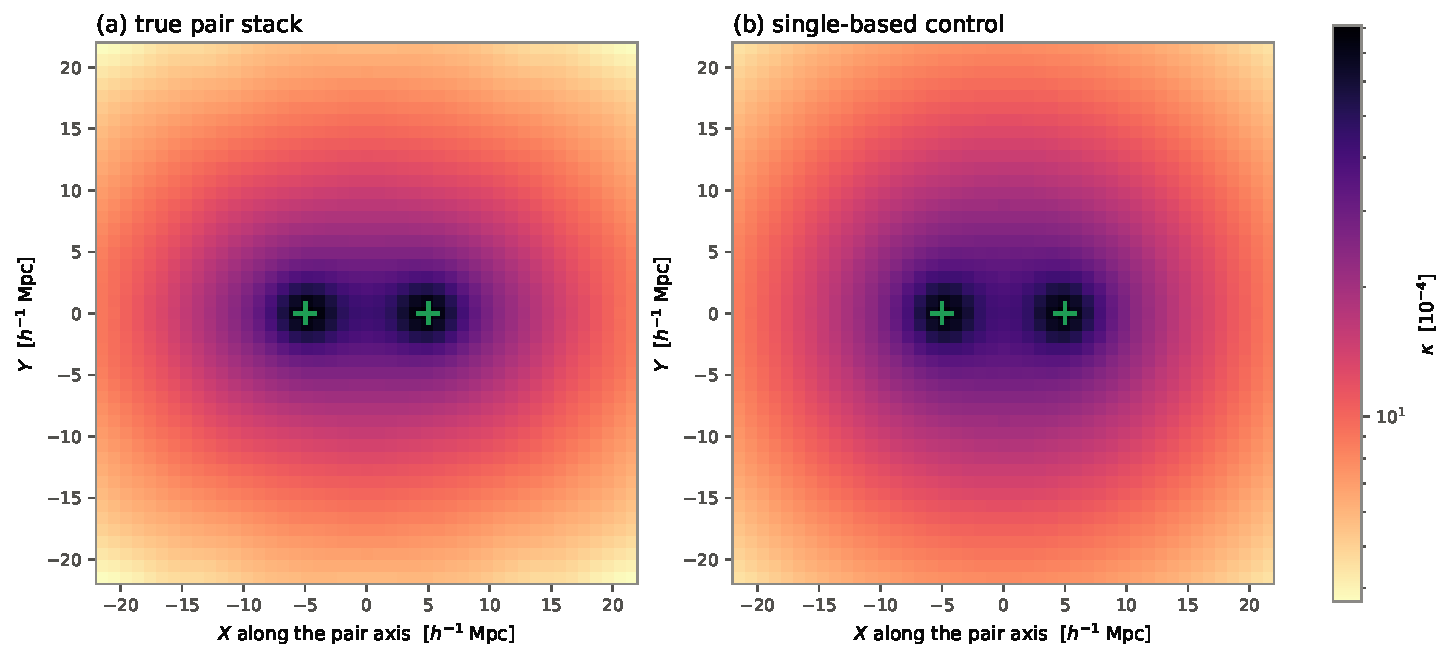
\includegraphics[width=0.9\linewidth]{Figure/sim_pair_vs_control_maps_sep10.pdf}
  \caption{Mock pair stack at $r_{\perp}=10\,\hinvMpc$ (left) and its
  unit-amplitude control, Equation~(\ref{eq:control}) (right), on a common
  color scale.}
  \label{fig:sim_pair_vs_control}
\end{figure*}

\begin{figure*}
  \centering
  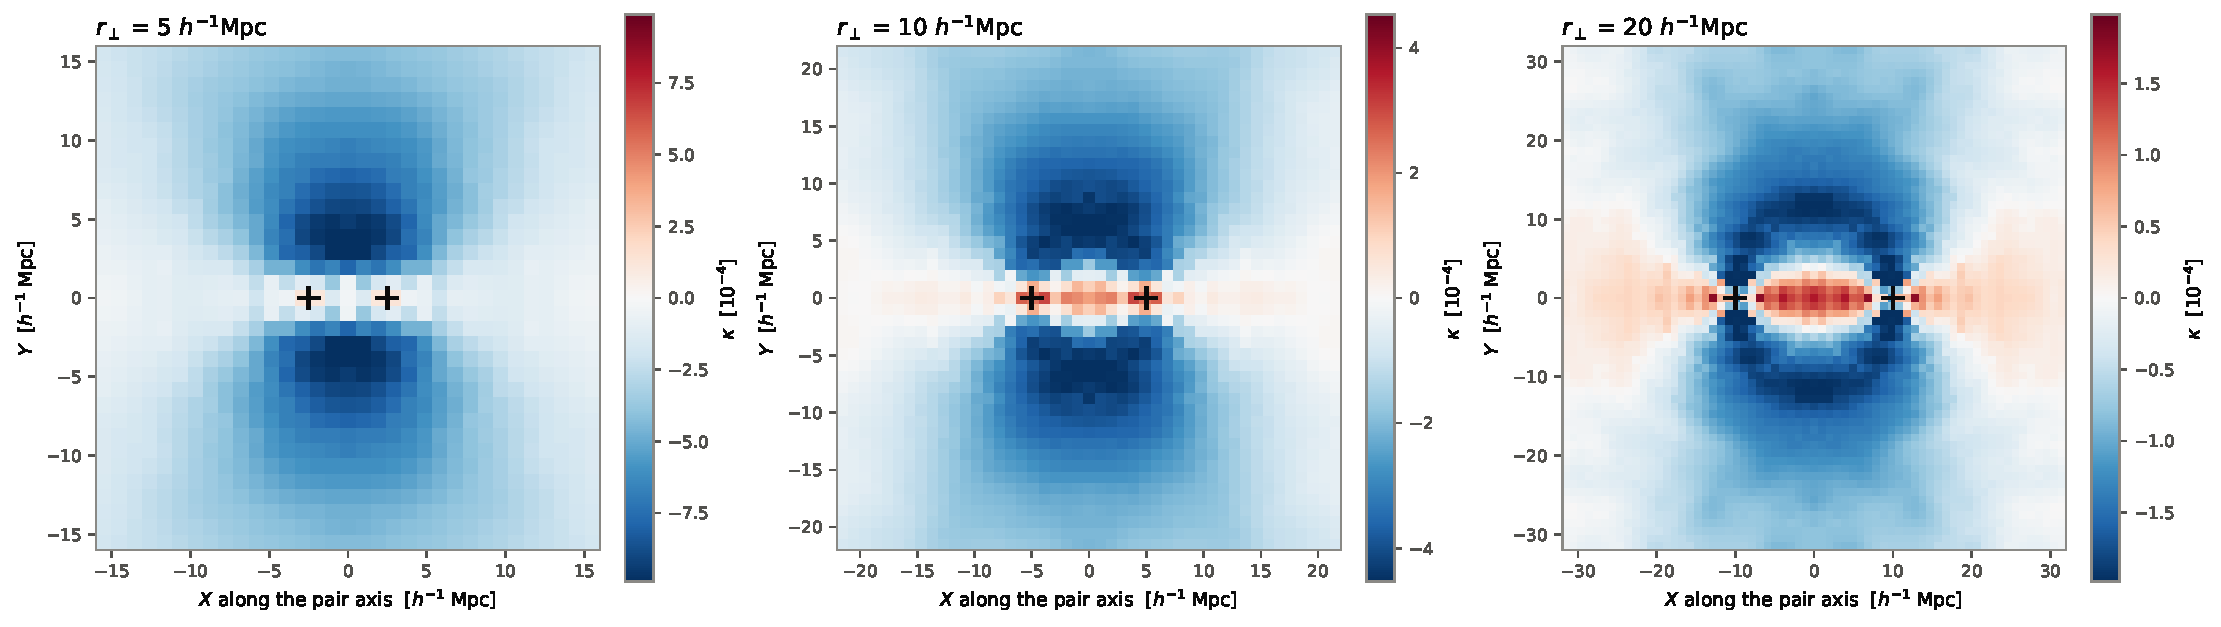
\includegraphics[width=0.9\linewidth]{Figure/sim_quadrupole_diff_maps.pdf}
  \caption{Mock residual maps $F$ at $r_{\perp}=5$, $10$, and $20\,\hinvMpc$
  (left to right), showing the ridge along the pair axis and the deficit
  perpendicular to it. Galaxy positions are marked.}
  \label{fig:sim_residual_maps}
\end{figure*}

Figure~\ref{fig:sim_band_profiles} shows the band profiles. The bridge
excess in the mock is
$\left(6.32\pm0.36,\ 4.91\pm0.21,\ 2.18\pm0.12\right)\times10^{-4}$ at
$r_{\perp}=5$, $10$, and $20\,\hinvMpc$. The corresponding $25$-block
jackknife signal-to-noise ratios are $17.7$, $22.9$, and $18.1$.
The decrease is consistent with a lower connected-pair fraction and lower
mean bridge density at larger separation. The mock residual also contains an
approximately isotropic component at the galaxy positions and an anisotropic
component along the pair axis.
% TODO: quote the mock residual at the halo positions and the midpoint kappa.

\begin{figure*}
  \centering
  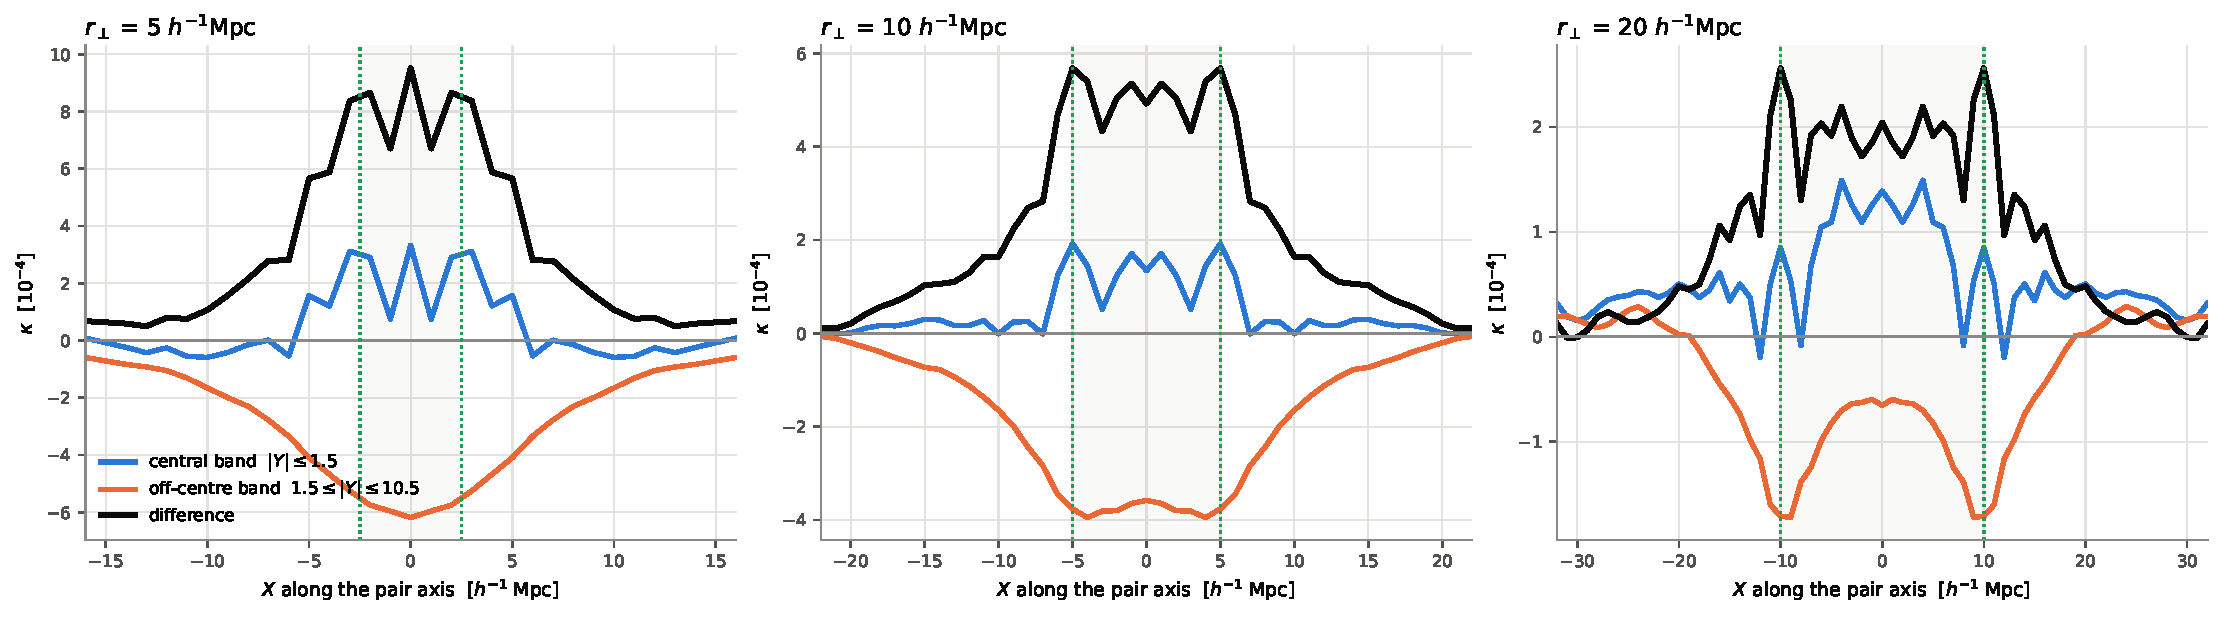
\includegraphics[width=0.9\linewidth]{Figure/sim_band_profiles_all_seps.pdf}
  \caption{Central-band mean, off-center-band mean, and their difference
  $B(X)$ for the mock residual maps at the three separations. The shaded
  window is $|X|\leq0.35\,d$.}
  \label{fig:sim_band_profiles}
\end{figure*}

The non-physical mock pairs show no bridge in any line-of-sight band,
confirming that the control does not itself generate a ridge.
% TODO: per-band residual bridge excess +/- error from nonphysical_pair_test_*.csv.
The line-of-sight sweep motivates the production cuts: at
$r_{\perp}=5\,\hinvMpc$ the bridge signal first rises and then falls as the
cut is widened, while at $10\,\hinvMpc$ it falls.
% TODO: completeness / interloper fraction / sensitivity per cut from rpar_scan.csv and los_sweep_summary.csv.

\section{Results}
\label{sec:results}

\subsection{Observed stacks}
\label{sec:obs_stacks}

The three BOSS samples contain $217{,}702$, $459{,}051$, and
$1{,}282{,}969$ pairs at $r_{\perp}=5$, $10$, and $20\,\hinvMpc$.
Figure~\ref{fig:boss_maps} shows the corrected single stack and the three
corrected pair stacks. Figure~\ref{fig:obs_vs_sim_maps} compares the
observed residual maps with the simulated ones. The observed maps contain a
broad axis-aligned excess and off-axis deficit, but these features have low
signal-to-noise in the Planck reconstruction.

\begin{figure*}
  \centering
  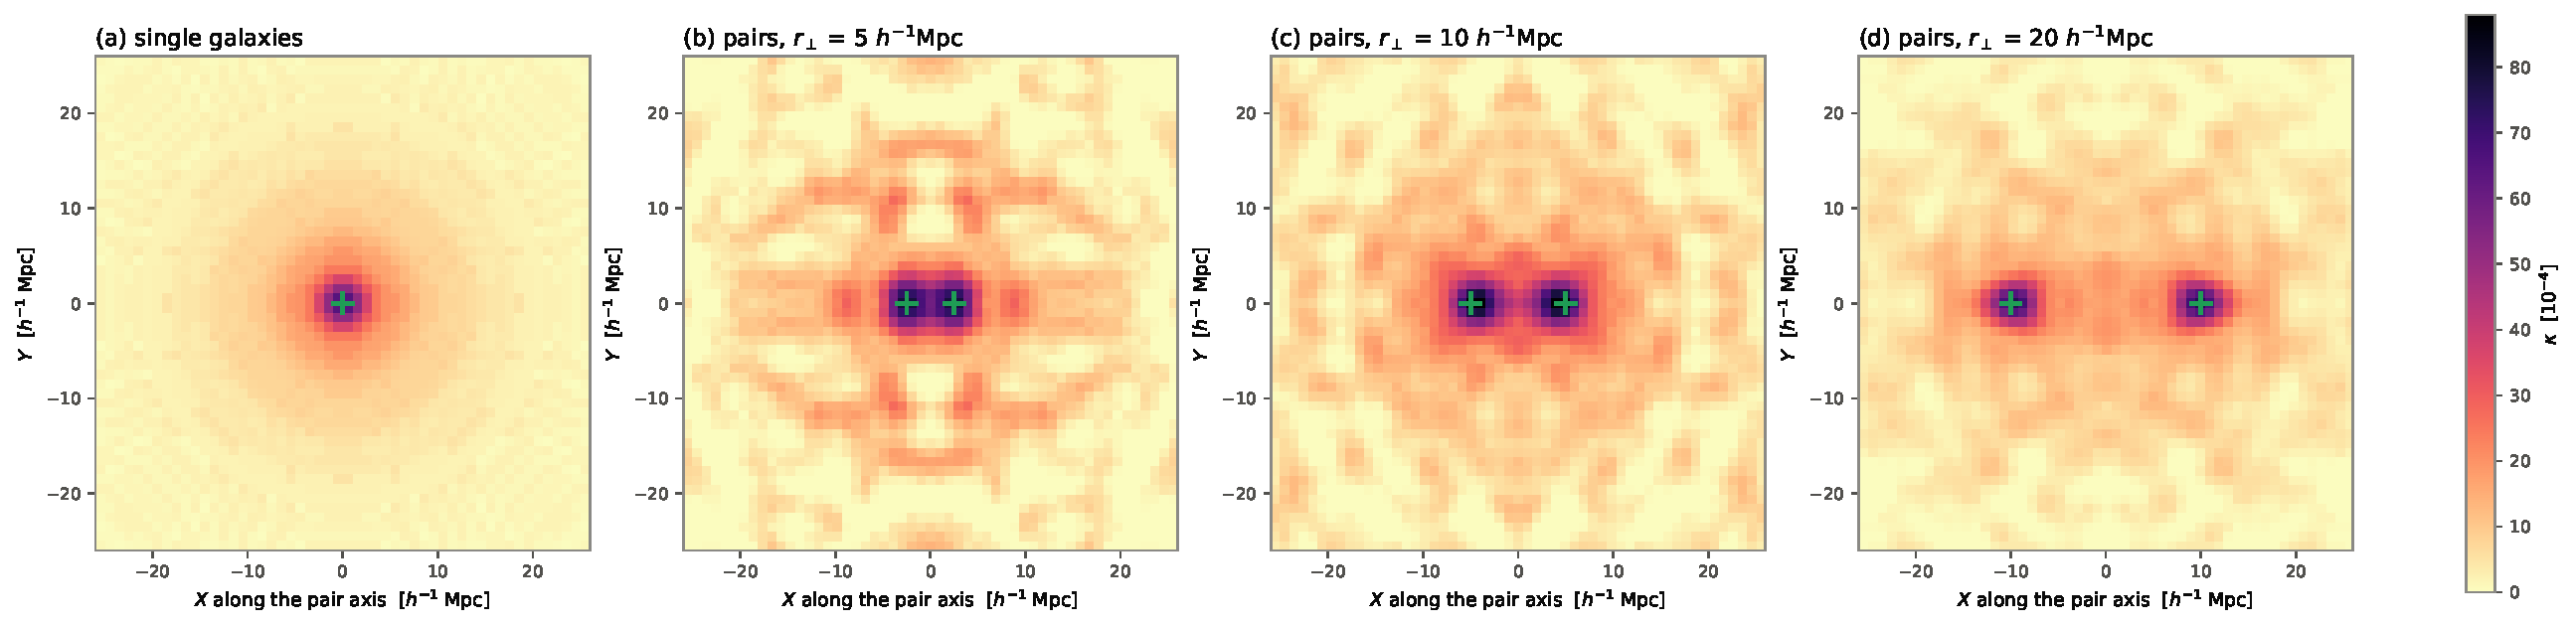
\includegraphics[width=0.9\linewidth]{Figure/boss_single_and_pair_maps.pdf}
  \caption{Corrected BOSS single-galaxy stack (left) and corrected pair
  stacks at $r_{\perp}=5$, $10$, and $20\,\hinvMpc$.}
  \label{fig:boss_maps}
\end{figure*}

\begin{figure*}
  \centering
  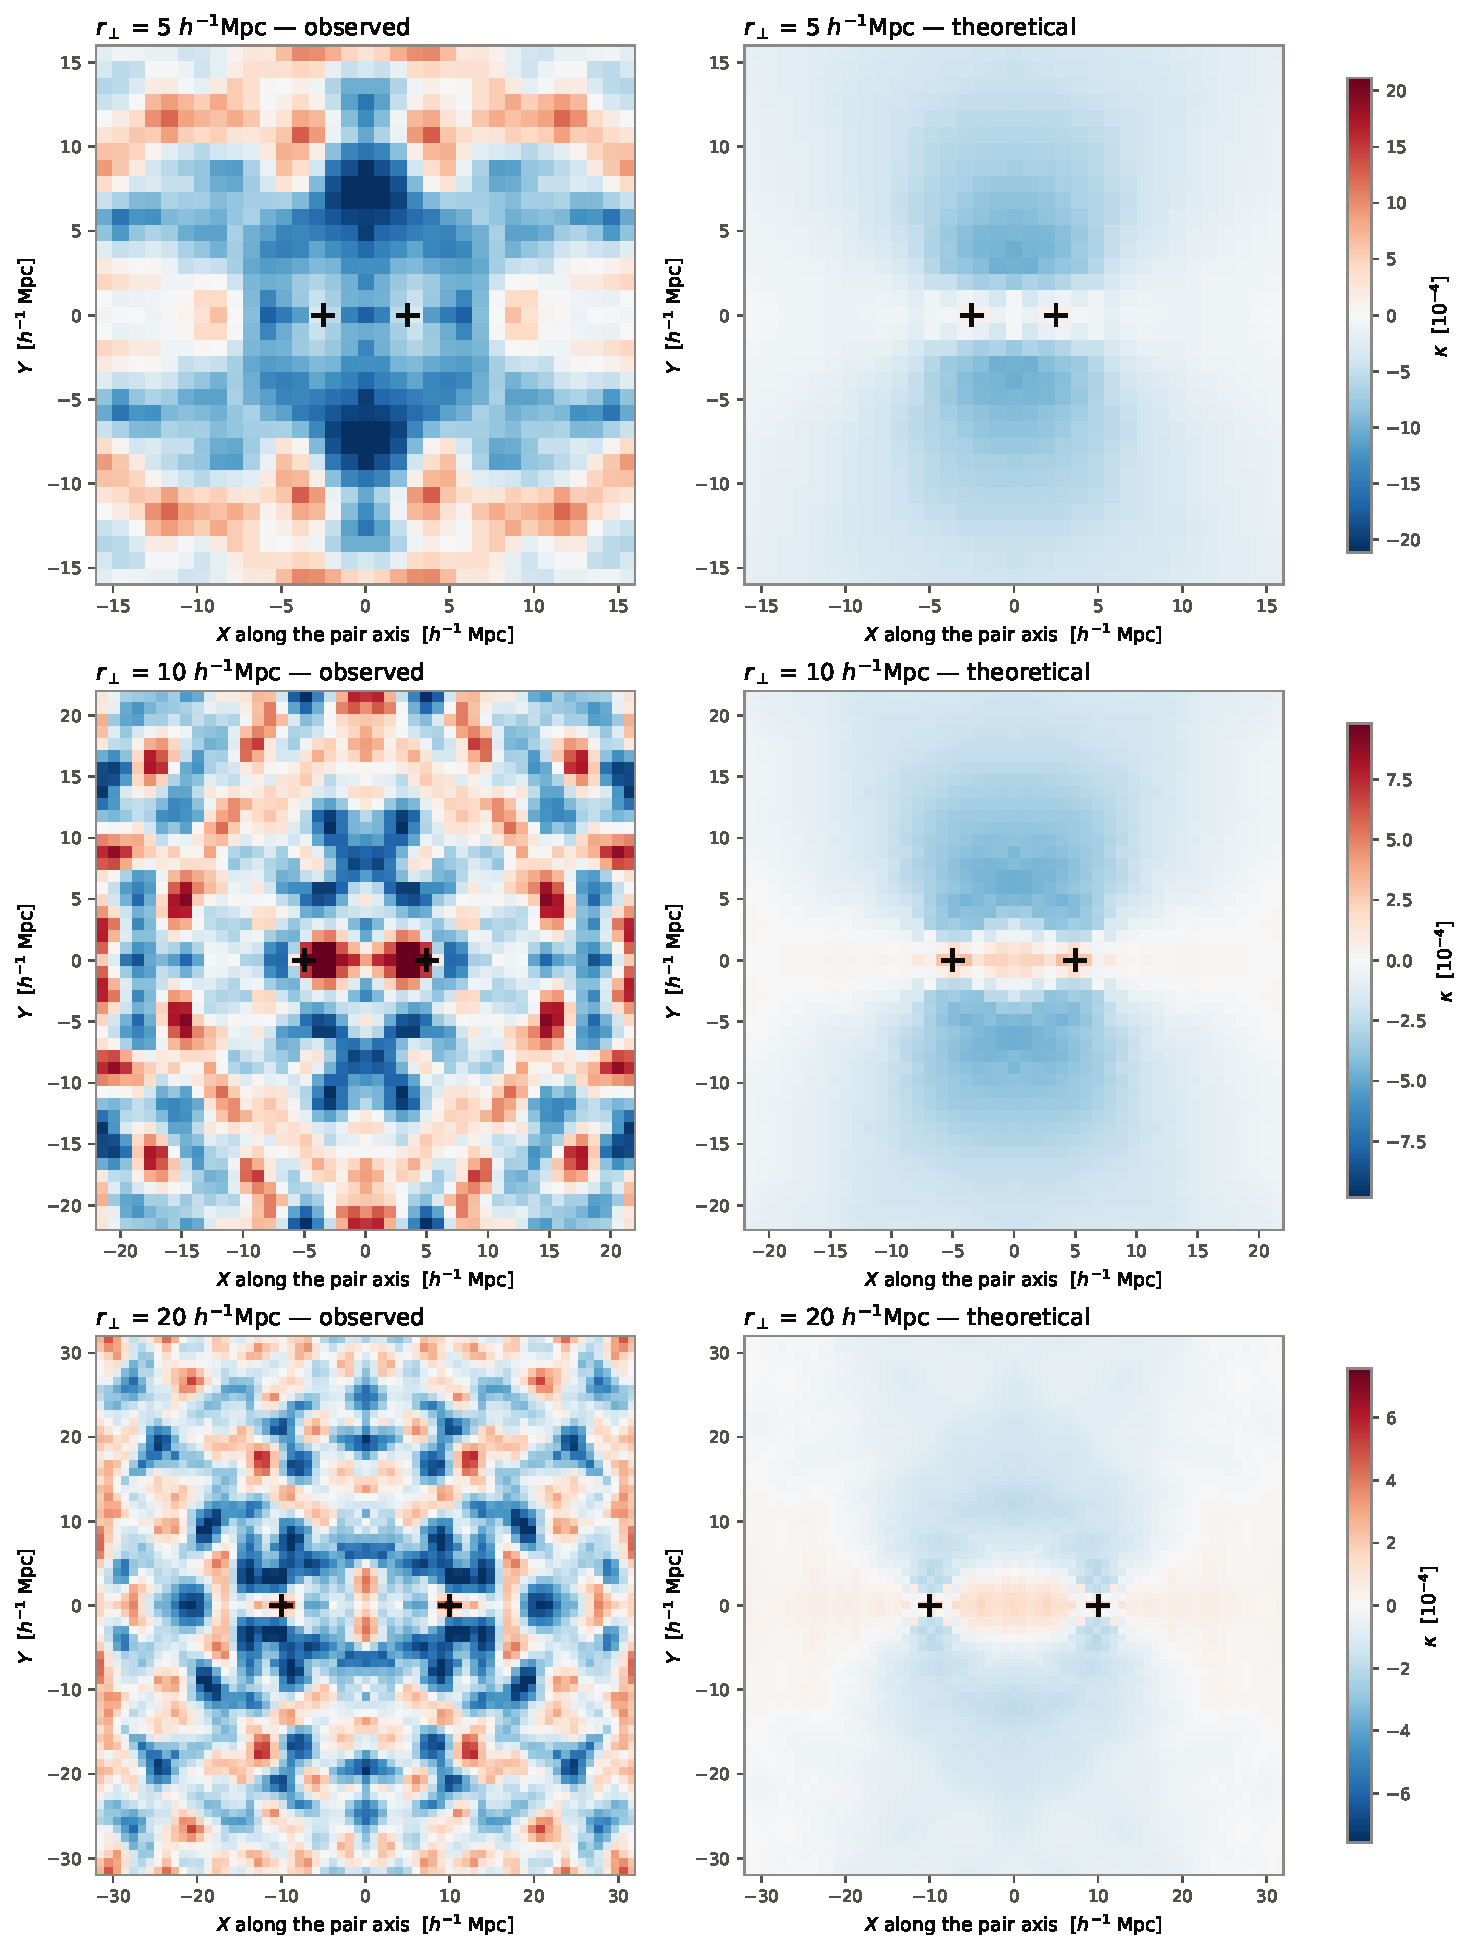
\includegraphics[width=0.7\linewidth]{Figure/obs_vs_sim_quadrupole_maps.pdf}
  \caption{Observed (left) and simulated (right) residual maps at
  $r_{\perp}=5$, $10$, and $20\,\hinvMpc$ (top to bottom), on a common
  color scale per row.}
  \label{fig:obs_vs_sim_maps}
\end{figure*}

\subsection{Bridge convergence}
\label{sec:bridge}

Table~\ref{tab:bridge} lists the bridge excess in each sample with its
jackknife error, beside the mock prediction in the same statistic.
Figure~\ref{fig:band_profiles_obs_sim} overlays the observed band profiles
on the mock prediction.

\begin{table}
  \centering
  \caption{Bridge excess, Equation~(\ref{eq:band}) averaged over
  $|X|\leq0.35\,d$, for the three BOSS samples, with the mock prediction in
  the same statistic. Observed errors are from the $287$-region delete-one
  jackknife with the control rebuilt in every realization; mock errors from
  the $25$-block jackknife. The final column is the observed-minus-mock
  difference divided by the quadrature sum of their errors.}
  \label{tab:bridge}
  \begin{tabular}{cccccc}
    \hline
    $r_{\perp}$ & $N_{\rm pairs}$ & Observed & S/N & Mock & Obs.$-$Mock \\
    $[\hinvMpc]$ & & $[10^{-4}]$ & & $[10^{-4}]$ & $[\sigma]$ \\
    \hline
    5  & $217{,}702$   & $5.38\pm9.08$  & $0.6$ & $6.32\pm0.36$ & $-0.1$ \\
    10 & $459{,}051$   & $11.91\pm5.10$ & $2.3$ & $4.91\pm0.21$ & $+1.4$ \\
    20 & $1{,}282{,}969$ & $1.24\pm2.22$  & $0.6$ & $2.18\pm0.12$ & $-0.4$ \\
    \hline
  \end{tabular}
\end{table}

\begin{figure*}
  \centering
  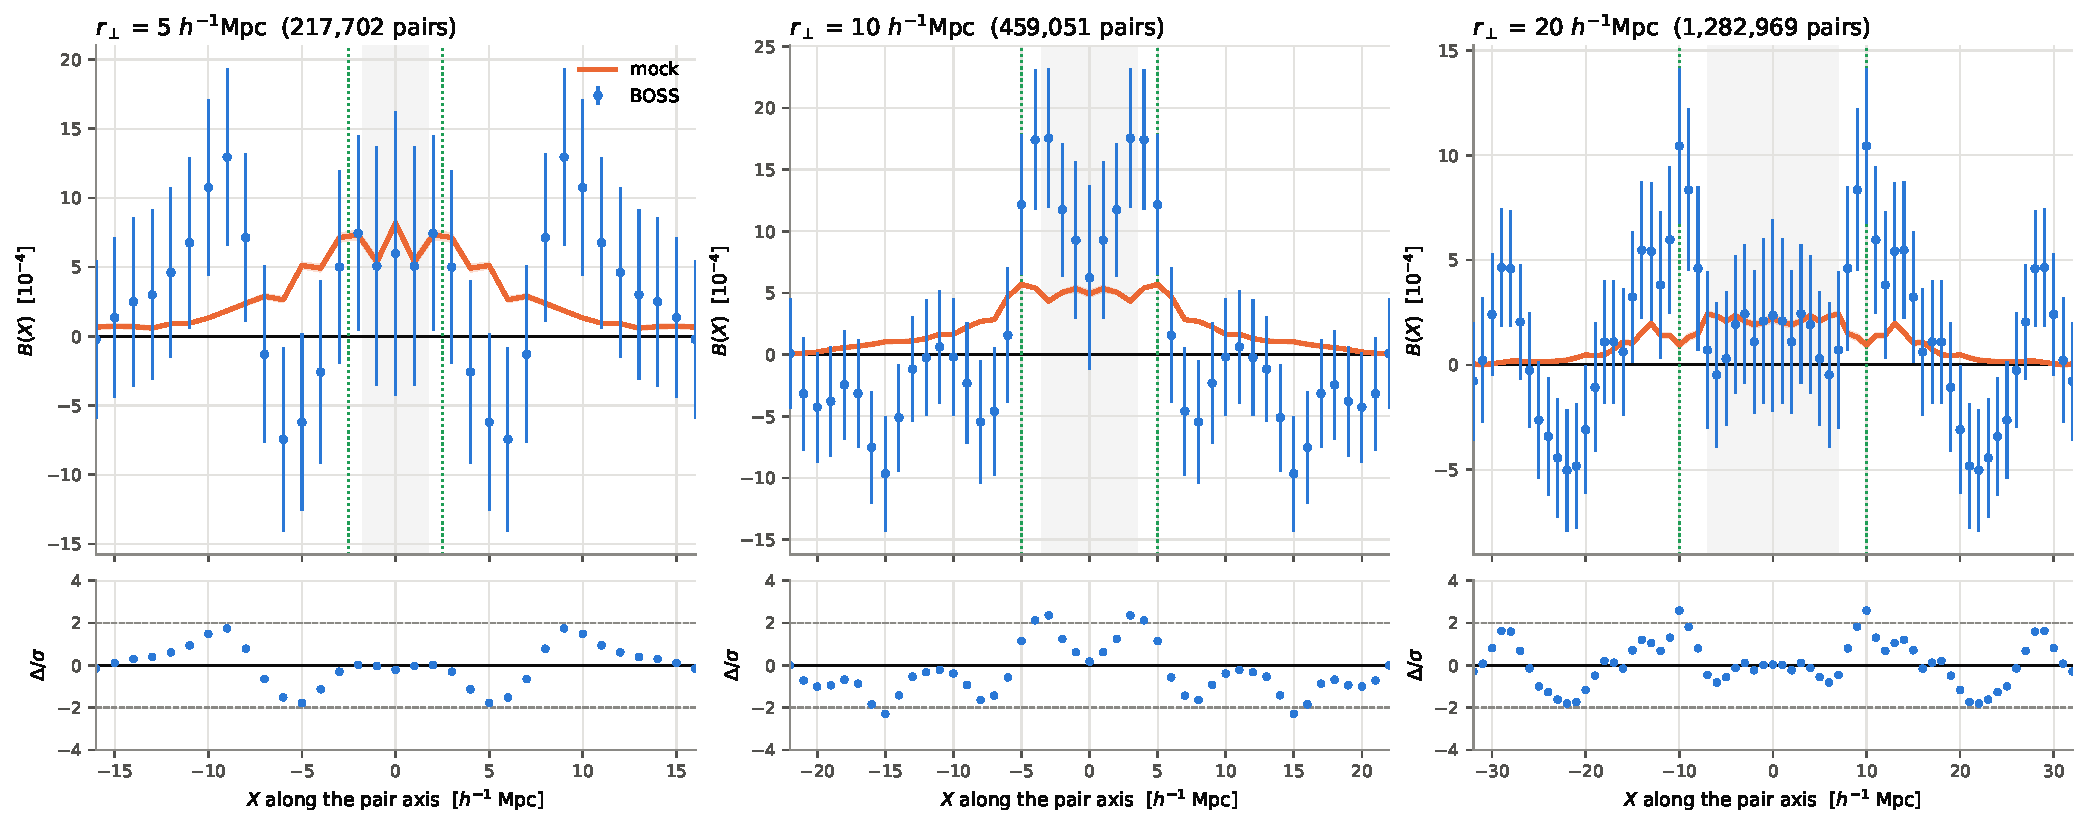
\includegraphics[width=0.9\linewidth]{Figure/band_profiles_obs_vs_sim.pdf}
  \caption{Observed band profile $B(X)$ with jackknife errors (points) and
  the mock prediction with its box-jackknife band (shaded) at the three
  separations. The observed errors are delete-one jackknife over the
  $287$ sky patches; the mock band is the $25$-block box jackknife, with
  the superposed-singles control held fixed across realizations. Gray marks
  the bridge window $|X| \leq 0.35\,d$; dotted green lines mark the galaxy
  positions.
  Lower panels: difference in units of the observed error, with dashed
  guides at $\pm2$. The mock pairs are selected in the same
  transverse bins as BOSS at all three separations. The mock band is
  statistical only: it is the $25$-block scatter of a single realization and
  excludes the uncertainty in the HOD.}
  \label{fig:band_profiles_obs_sim}
\end{figure*}

No bridge excess exceeds $3\sigma$. The $10\,\hinvMpc$ sample has a positive
excess of $2.3\sigma$ and lies $1.4\sigma$ above the mock prediction; the
other two bridge excesses are consistent with zero.
A $\chi^{2}$ test of the compressed $22$-element profile against zero with
the full covariance gives $\chi^{2}=35.0$, $20.7$, and $32.4$ for $22$
degrees of freedom (nominal $p=0.04$, $0.54$, and $0.07$). The $p=0.04$
result at $5\,\hinvMpc$ is a full-profile departure from zero, not a bridge detection:
the test includes the bins containing the galaxies.

Fitting the amplitude of the mock residual profile to the observed profile with
Equation~(\ref{eq:amplitude}) over the full $22$-element vector returns
$A=1.47\pm0.36$, $1.07\pm0.49$, and $1.60\pm0.57$, at $4.1$, $2.2$, and
$2.8\sigma$.
At $10$ and $20\,\hinvMpc$, bins around the galaxies contribute $59$ and
$44$ percent of the fitted response. At $5\,\hinvMpc$, the
$4\,\hinvMpc$ binning places the galaxy positions in the only bridge bin,
so their contributions cannot be separated. The full-profile amplitude
is therefore not a bridge amplitude. Restricting the fit to the bridge window
$|X|\leq0.35\,d$ gives $A=1.97\pm0.58$, $1.81\pm0.84$, and $0.71\pm0.95$, at
$3.4$, $2.1$, and $0.7\sigma$. These significances differ from the bridge
excesses in Table~\ref{tab:bridge} because the fit treats the central and
off-center bands as separate data elements, whereas the bridge statistic
uses their difference. The $5\,\hinvMpc$ fit still contains the unresolved
galaxy bin, and beam-convolved halo signal can enter the bridge window at all
three separations. We therefore use these fits as profile diagnostics rather
than bridge detections. A nested test that adds a free constant to the full
profile leaves the amplitudes unchanged and returns offsets of
$\left(-1.6,\ +0.4,\ +0.2\right)\times10^{-4}$, consistent with zero.

\subsection{Comparison with the simulation and with previous work}
\label{sec:compare}

The direct data--mock comparison is the bridge statistic in
Table~\ref{tab:bridge}, for which both maps use the same bands, bridge window,
and smoothing. The observed uncertainties exceed the predicted bridge
amplitudes at all three separations, and the measurements are consistent with
both zero and the mock.

A $95$ percent upper limit on the bridge excess can be converted to a surface
density using $\Sigma_{\rm crit}$ and then to a linear mass density over the
bridge length.
% TODO: compute the upper limits and compare them with Epps & Hudson (2017) and de Graaff et al. (2019).

The residual maps also test whether the control describes the paired haloes.
The observed residual map peaks at the galaxy positions at about
$2\times10^{-3}$, compared with $0.9\times10^{-3}$ in the mock.
% CHECK: values from the fit_sim_template.py docstring; confirm from checked-in output.
If confirmed, this difference means that paired CMASS galaxies have a larger
excess over the average CMASS galaxy than paired mock galaxies have over the
average mock galaxy. A central-only HOD with a soft mass threshold may produce
a different pair selection from the observed sample, which includes
satellites and a stellar-mass selection. The corrected single-galaxy profile
also lies below the matched mock prediction at large radius.
% CHECK: fit_sim_template.py docstring; compare_boss_mock_profile.py retracted earlier significance values.
These comparisons constrain the isotropic residual from which the
axis-aligned signal is separated; they do not directly measure the bridge
statistic because Equation~(\ref{eq:band}) subtracts the off-center band.
% TODO: compare corrected single profiles in the 10--20, 15--25, and 20--40 h^-1 Mpc bands with jackknife errors.

\citet{deGraaff2019} measured
$\bar\kappa=(5.8\pm3.1)\times10^{-4}$ in the bridge region of pairs pooled
over $6$--$14\,\hinvMpc$. Their statistic differs from ours in four ways:
pairs are rescaled to unit separation before stacking, the bridge region is
defined on the rescaled grid, the halo model is fitted to the pair stack in
a $60^\circ$ sector about the direction perpendicular to the pair axis, and
the map is smoothed to $10$ arcmin. Their central value is numerically close
to our $10\,\hinvMpc$ result, but the two estimators are not identical. Their
sample contains about $2.2$ times as many pairs as our $10\,\hinvMpc$
sample; independent-pair scaling alone would reduce the error by a factor of
$1.5$.
Pooling our three samples with inverse-variance weights would provide an
approximate comparison, but it would remain a different estimator from that
of \citet{deGraaff2019}.
% TODO: quote the pooled value if this comparison is retained.

\subsection{Robustness tests}
\label{sec:robust}

\paragraph{Smoothing.} Figure~\ref{fig:smoothing_scan} compares the observed
$8$- and $6$-arcmin results at all three separations and the $4$-arcmin
result at $5$ and $10\,\hinvMpc$. The bridge signal-to-noise values for
$8$, $6$, and $4$ arcmin are $(0.6,1.2,2.2)$ at $5\,\hinvMpc$ and
$(2.3,2.4,1.1)$ at $10\,\hinvMpc$; at $20\,\hinvMpc$ the $8$- and
$6$-arcmin values are $0.6$ and $0.5$. We retain $8$ arcmin as the common
smoothing scale and do not tune it separately for each separation.

\begin{figure}
  \centering
  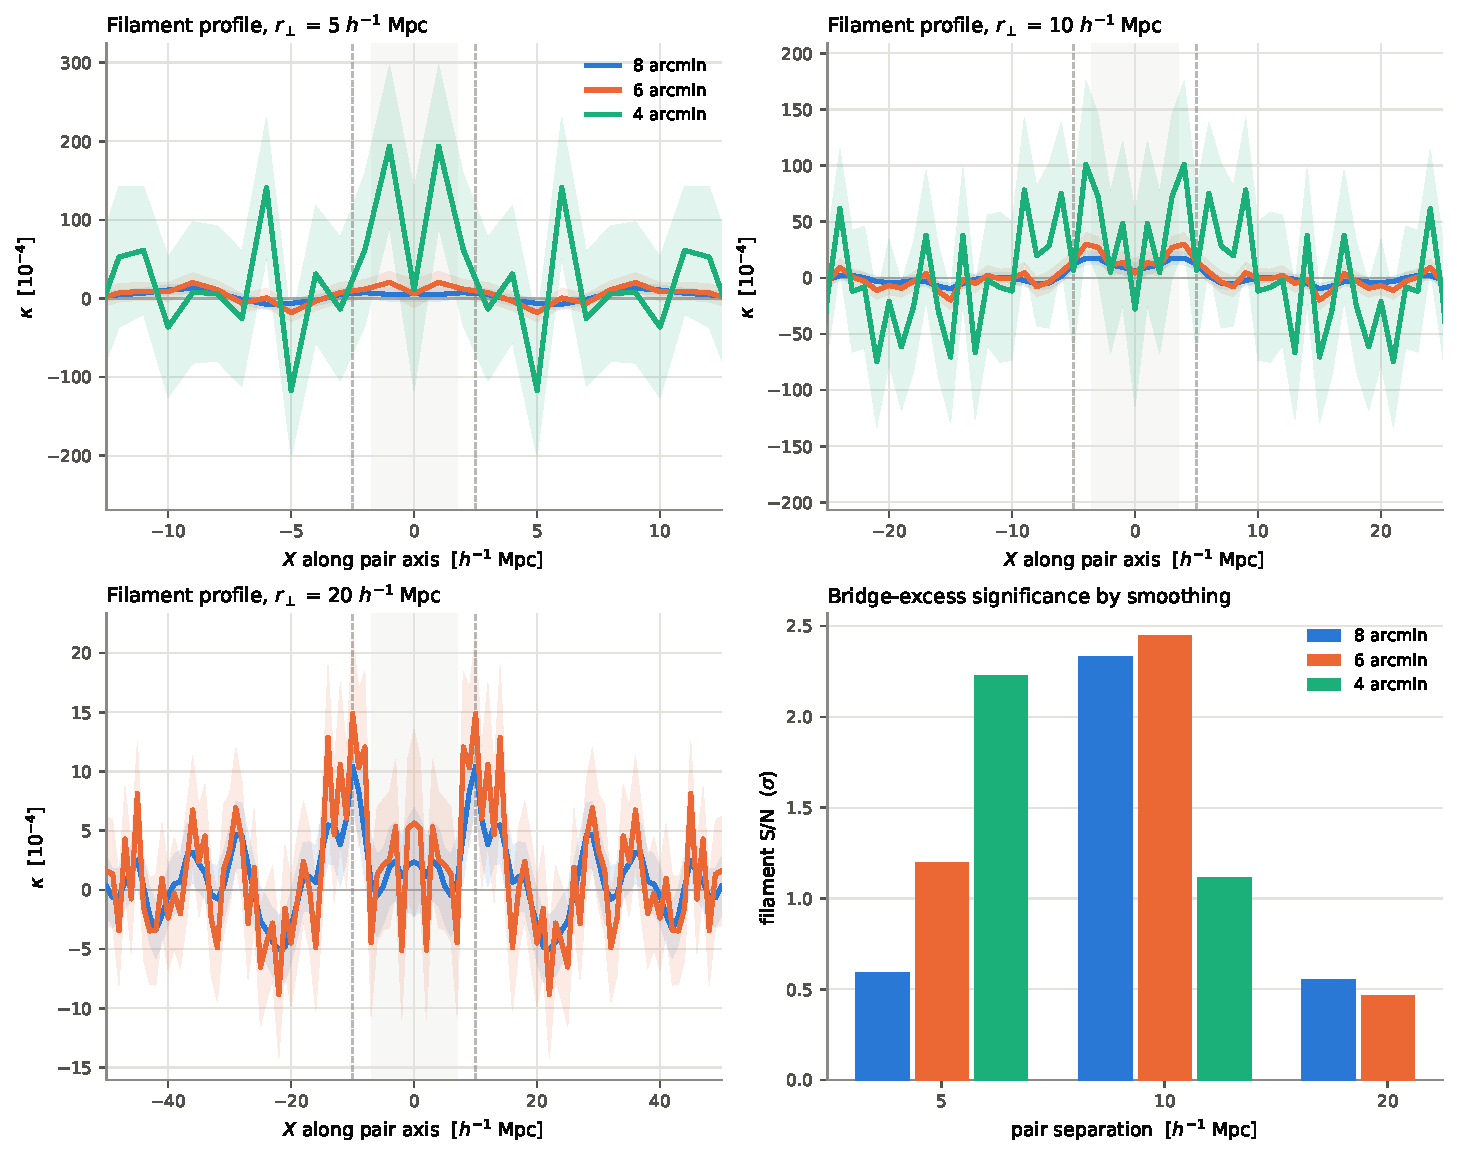
\includegraphics[width=\linewidth]{Figure/filament_snr_vs_smoothing.pdf}
  \caption{Observed bridge profiles and signal-to-noise for the available
  smoothing FWHM values. The $4$-arcmin stack is unavailable at
  $20\,\hinvMpc$.}
  \label{fig:smoothing_scan}
\end{figure}

\paragraph{Weighting.} The effect of removing the lensing-efficiency weight
from the single stacks has not yet been quantified.
% TODO: report the changes in the control and bridge excess.
Combining the two caps by an equal-weight average instead of the joint stack
produced the apparent dip reported in earlier versions of this analysis.
% TODO: report the shift in the corrected single profile at 20 h^-1 Mpc.

\paragraph{Random-pair sample.} Replacing the full random catalog by a
10 percent subsample shifts the $10\,\hinvMpc$ bridge excess by
$5\times10^{-4}$, comparable to the signal, which is why the full randoms
are required. % CHECK: combine_filament_jackknife.py docstring.

\paragraph{Fitted control.}
% UNVERIFIED: align this description with band_core_tail_control.py and add checked-in results.
As an alternative to the unit-amplitude control, we split the single-galaxy
profile into core and tail components and fit their amplitudes outside the
pair. On the mock this control drives the bridge excess to zero at all three
separations, whereas the unfitted control recovers the known bridge. The
fitted control therefore absorbs axis-aligned signal, and we do not use it
for the headline measurement.
% TODO: quote mock and observed bridge excess under the fitted control beside the unfitted values.
